\documentclass[11pt,a4paper]{report}

% === Codifica e font ===
\usepackage[utf8]{inputenc}
\usepackage[T1]{fontenc}
\usepackage{lmodern}

% === Lingua ===
\usepackage[italian]{babel}

% === Margini e geometria ===
\usepackage{geometry}
\geometry{a4paper, margin=2.5cm}

% === Colori ===
\usepackage{xcolor}
\definecolor{headergray}{gray}{0.9}
\definecolor{rowgray}{gray}{0.97}
\definecolor{upmred}{RGB}{200, 16, 46}  % Colore istituzionale

% === Tabelle e layout ===
\usepackage{array}
\usepackage{tabularx}
\usepackage{booktabs}
\usepackage{longtable}
\usepackage{makecell}
\renewcommand\theadfont{\bfseries}
\usepackage[table,xcdraw]{xcolor}

% === Stile documento ===
\usepackage{graphicx}
\usepackage{caption}
\usepackage{ragged2e}
\usepackage{multicol}
\usepackage{enumitem}

% === Hyperlink ===
\usepackage{hyperref}
\hypersetup{
    colorlinks=true,
    linkcolor=upmred,
    urlcolor=blue
}

% === Intestazioni e piè di pagina ===
\usepackage{fancyhdr}
\pagestyle{fancy}
\fancyhf{}
% Intestazione: a sinistra il titolo del capitolo, a destra nome università
\fancyhead[L]{\small \nouppercase{\leftmark}} 
\fancyhead[R]{\small Università Politecnica delle Marche}
% Piè di pagina: numero centrato
\fancyfoot[C]{\thepage}

% === Titolo principale ===
\begin{document}

\begin{titlepage}
  \vspace*{-1cm}
  \begin{center}
    \textbf{\textcolor{upmred}{\LARGE UNIVERSITÀ POLITECNICA DELLE MARCHE}}\\[0.3cm]
    \large Corso di Laurea Triennale in Ingegneria Informatica e dell'Automazione
    \vspace{0.5cm}

    
\includegraphics[width=0.5\textwidth]{logo.jpg} \\[0.7in]

    {\Large\textbf{\textcolor{upmred}{UniMoL (University Molecular Laboratory)}}}
    \vspace{0.4in}

\noindent
\begin{minipage}[t]{0.48\textwidth}
  {\Large\textcolor{upmred}{RELATORI:} \\[0.3cm]
  Prof. Ursino Domenico \\
  Prof. Davide Traini}
\end{minipage}
\hfill
\begin{minipage}[t]{0.48\textwidth}
  {\Large\textcolor{upmred}{TESINA DI:} \\[0.3cm]
  Letizia Lucrezia Mulieri \\
  Nicolò Palmerini \\
  Santarelli Paolo}
\end{minipage}


    \vspace{1in}

    {\Large ANNO ACCADEMICO 2024/2025}
  \end{center}
\end{titlepage}

\tableofcontents


\chapter*{Introduzione}
\addcontentsline{toc}{chapter}{Introduzione}
\markboth{INTRODUZIONE}{}
L’ingegneria del software riveste un ruolo fondamentale nello sviluppo di soluzioni affidabili, scalabili e manutenibili, con la 
continua e cresecente evoluzione dei sistemi informatici. \\ Lo scopo del presente elaborato è quello di mostrare le fasi di analisi, 
progettazione e sviluppo di un'applicazione software a partire dalla raccolta dei requisiti fino alla fase di test e validazione.
L'obiettivo principale del progetto è stato quello di realizzare una piattaforma web in grado di gestire un laboratorio di biologia 
molecolare di un'università e in base alla tipologia di utente offrire diversi servizi.\\ Nel corso della tesina sono stati inseriti tutti i 
manufatti realizzati al fine di ricoprire tutte le fasi dello sviluppo software, inclusa l'analisi dei requisiti, la progettazione 
dell’architettura e dei componenti, 
l’implementazione e la validazione del sistema. Verranno inoltre illustrate le scelte tecniche adottate.\\ Il progetto rappresenta 
un'opportunità concreta per mettere in pratica le metodologie apprese durante il corso, con particolare attenzione alla qualità del 
software, alla documentazione e alla collaborazione in un contesto di sviluppo strutturato.


\chapter{Descrizione del progetto}
\section{Descrizione in linguaggio naturale}
Il progetto proposto consiste nella realizzazione di una piattaforma web che consente di gestire un laboratorio di biologia molecolare di un’università.
\\\\In particolare, il software sarà in grado di soddisfare diversi servizi in base alla tipologia di utente (professore, ricercatore, studente, tecnico di laboratorio): \\
•	Prenotazione del laboratorio (locale fornito di apposite installazioni e apparecchi per studi, ricerche, esperimenti)\\
•	Iscrizione alle attività didattiche\\
•	Gestione dell’attrezzatura e dei materiali adoperati nelle attività laboratoriali
\subsubsection{Gestione laboratorio}
Il laboratorio è disponibile durante il corso dell’anno accademico, seguendo gli orari di apertura della facoltà, dalle ore 07:30 alle ore 19:00. Non è possibile accedervi e prenotarsi nei giorni festivi. \\
Le prenotazioni possono essere effettuate solamente da professori e ricercatori. \\
Il numero massimo di persone consentito è di 20 (fra professori, ricercatori e studenti, esclusi i tecnici di laboratorio). \\
La strumentazione e i materiali messi a disposizione dal laboratorio posso essere utilizzati se esplicitamente indicato all’interno della prenotazione. 
Esistono due tipologie di prenotazione: \\
-	Lezione (possono essere effettuate dal professore) \\
-	Attività (possono essere effettuare dal ricercatore)\\
Il numero massimo di ore durante il quale si può usufruire del laboratorio per la tipologia lezione è di 2 ore. La tipologia di prenotazione attività non ha un limite massimo di ore (non è consentito oltrepassare il consueto orario di apertura). \\
La tipologia di prenotazione lezione consente di fissare un calendario per l’attività didattica, specificando i giorni e gli orari preposti. \\
Il ricercatore ha la possibilità di prenotare il laboratorio per la tipologia di prenotazione: attività. Al momento della prenotazione è consentito specificare giorno e orari prestabiliti, con la possibilità di indicare attrezzature e materiali richiesti per le suddette attività laboratoriali. Inoltre, è consentito indicare il numero massimo di persone che possono prendere parte all’attività (senza superare la capienza massima, escludendo i tecnici). \\
Al ricercatore è consentito eliminare una prenotazione. Le prenotazioni per entrambe le tipologie devono essere effettuare almeno 5 giorni prima della data di prenotazione stessa e possono essere modificare entro i 3 giorni prima della data scelta (con possibilità di modificare orario, giorno o eventualmente eliminare l’attività didattica).\\ 
Non è consentito prenotare più di una attività all’interno della stessa fascia oraria(es. non è possibile avere una lezione ed anche un esperimento relativi allo stesso orario). 
\subsubsection{Gestione utente }
Ad ogni utente è consentito l’accesso alla piattaforma tramite credenziali fornite dall’ateneo di appartenenza (codice identificativo e password). \\\\
Gli utenti che possono accedere al sistema sono suddivisi in 4 categorie:\\
-	Professore\\
-	Ricercatore\\
-	Studente\\
-	Tecnico di laboratorio
\subsubsection{Gestione professore}
L’utente professore ha la possibilità di specificare al momento della prenotazione la tipologia fra: attività e lezione. Inoltre, il professore può fornire un elenco di corsi al quale lo studente può iscriversi. Il professore può gestire i suoi corsi, inserire un calendario delle lezioni (indicando giorni e orari preposti), visualizzare gli studenti iscritti ai corsi. 
\subsubsection{Gestione studente}
Lo studente può segnarsi per una o più attività didattiche (tra lezioni e attività pratiche).\\
Il suddetto può eliminare una prenotazione per la tipologia attività entro 3 giorni prima dell’attività stessa. \\
Allo studente è consentito iscriversi a uno o più corsi messi a disposizione dei professori. In tal modo sarà automaticamente prenotato a tutte le lezioni inserite dal professore del corso stesso, con possibilità di disiscriversi entro il giorno prima della data della lezione. 
\subsubsection{Gestione tecnico}
Il tecnico di laboratorio gestisce gli strumenti e i materiali messi a disposizione dal laboratorio. Il tecnico deve visualizzare tutta la strumentazione disponibile e indicare eventuali malfunzionamenti della stessa; deve visualizzare l’elenco dei materiali (inventario) indicando quelli non disponibili per cui è necessario il rifornimento (da riordinare).
\vspace{1em} \\ Una procedura di backup del sistema viene eseguita automaticamente tutti i giorni alle ore 01:00 a.m. 


\newpage
\section{Glossario dei termini}

\renewcommand\cellalign{cc} % centratura orizzontale + verticale per makecell
\renewcommand\arraystretch{1.6} % aumenta lo spazio verticale tra righe

\begin{table}[!ht]
\centering
\begin{tabular}{|p{3.5cm}|p{3.5cm}|p{3cm}|p{3cm}|}
\hline
\makecell{\textbf{TERMINE}} & \makecell{\textbf{DESCRIZIONE}} & \makecell{\textbf{TIPO}} & \makecell{\textbf{SINONIMI}} \\
\hline
\makecell{UTENTE}  &  Chi accede al sistema e non ha potere di gestione del software  & TECNICO &  - \\
\hline
\makecell{PROFESSORE} & Dipendente dell'università, può prenotare l'aula, eliminare la prenotazione e gestire materiali e strumenti per attività laboratoriali & BUSINESS & DOCENTE, INSEGNANTE \\
\hline
\makecell{RICERCATORE} & Dipendente dell'università, può prenotare l'aula, eliminare la prenotazione e gestire materiali e strumenti per attività laboratoriali & BUSINESS & - \\
\hline
\makecell{TECNICO} & Dipendente dell'università, può acquistare materiali e strumenti per il laboratorio e gestire l'inventario & BUSINESS & - \\
\hline
\makecell{STUDENTE} & Persona che può iscriversi ai corsi dei professori, prenotarsi alle attività laboratoriali dei ricercatori e disiscriversi da un corso & BUSINESS & MATRICOLA \\
\hline
\end{tabular}
\caption{Glossario dei termini - Parte 1}
\end{table}

\vspace{1em}
\newpage
\begin{table}[!ht]
\centering
\begin{tabular}{|p{3.5cm}|p{3.5cm}|p{3cm}|p{3cm}|}
\hline
\makecell{\textbf{TERMINE}} & \makecell{\textbf{DESCRIZIONE}} & \makecell{\textbf{TIPO}} & \makecell{\textbf{SINONIMI}} \\
\hline
\makecell{IDENTIFICATIVO} & Sequenza di numeri e lettere assegnati ad un utente per identificarlo & TECNICO & ID, CODICE \\
\hline
\makecell{\\ATTIVITÀ \\LABORATORIALI} & Mansioni che possono essere svolte all'interno del laboratorio & BUSINESS & - \\
\hline
\makecell{MATERIALI} & Elementi ed oggetti utilizzati durante gli esperimenti & BUSINESS & ELEMENTI \\
\hline
\makecell{STRUMENTI} & Dispositivi utilizzati durante le attività laboratoriali & BUSINESS & DISPOSITIVI \\
\hline
\makecell{INVENTARIO} & Insieme di materiali e strumenti presenti nel magazzino & BUSINESS & - \\
\hline
\makecell{PRENOTAZIONE} & Atto mediante il quale vengono riservati uno o più servizi ad un utente in un certo periodo di tempo & BUSINESS & - \\
\hline
\makecell{LABORATORIO} & Struttura per attività didattiche & BUSINESS & - \\
\hline
\makecell{BACKUP} & Copia di sicurezza dei dati del sistema & TECNICO & - \\
\hline
\end{tabular}
\caption{Glossario dei termini - Parte 2}
\end{table}
\newpage

\chapter{Requisiti}
In questa sezione vengono analizzati i requisiti del sistema, evidenziando la suddivisione tra:
\begin{itemize}
  \item requisiti funzionali, ovvero le funzionalità desiderate per il sistema
  \item requisiti non funzionali, ovvero i vincoli che il sistema dovrà rispettare
\end{itemize}
È stata aggiunta una tabella per suddividere i requisiti in base alla priorità secondo il paradigma MoSCoW. Inoltre vengono mostrati i casi d'uso estratti dai requisiti funzionali e le relazioni che intercorrono con gli attori attraverso i diagrammi dei casi d'uso.
Per ogni diagramma vengono descritti i rispettivi casi d'uso secondo una tabella che ne evidenzia gli aspetti fondamentali. Infine  la matrice di mapping è stata inserita per evidenziare
il rapporto tra i requisiti e i rispettivi casi d'uso, generata tramite lo strumento di modellazione Enterprise Architect (con la quale sono stati realizzati tutti i diagrammi). 

\section{Requisiti Funzionali}
\begin{longtable}{>{\raggedright\arraybackslash}p{5cm} >{\raggedright\arraybackslash}p{10cm}}
\toprule
\rowcolor{headergray}
\textbf{Codice Requisito} & \textbf{Descrizione} \\
\midrule
\rowcolor{white}
RF-01 CRUD Attività & Il sistema dovrà gestire inserimento, visualizzazione, modifica e rimozione di una prenotazione di tipo attività \\
\rowcolor{rowgray}
RF-02 Iscrizione Attività & Il sistema dovrà permettere allo studente di iscriversi a un'attività (proposta da un ricercatore) \\
\rowcolor{white}
RF-03 Cancellazione Iscrizione Attività & Il sistema dovrà permettere allo studente di annullare l'iscrizione a un'attività \\
\rowcolor{rowgray}
RF-04 CRUD Strumento & Il sistema dovrà gestire l’inserimento, modifica, visualizzazione ed eventuale rimozione di uno strumento \\
\rowcolor{white}
RF-05 CRUD Materiale & Il sistema dovrà gestire l’inserimento, modifica, visualizzazione ed eventuale rimozione del materiale \\
\rowcolor{rowgray}
RF-06 CRUD Lezione & Il sistema dovrà gestire l’inserimento, la modifica, la visualizzazione e cancellazione di una prenotazione di tipo lezione \\
\rowcolor{white}
RF-07 Cancellazione Corso & Il sistema dovrà permettere al professore di eliminare un corso \\
\rowcolor{rowgray}
RF-08 Cancellazione Iscrizione Corso & Il sistema permetterà allo studente di disdire l'iscrizione ad un corso \\
\rowcolor{white}
RF-09 Iscrizione Lezione & Il sistema dovrà permettere allo studente di iscriversi a una determinata lezione \\
\rowcolor{rowgray}
RF-10 Visualizzazione Corsi & Il sistema dovrà permettere all'utente di visualizzare i corsi disponibili \\
\rowcolor{white}
RF-11 Inserisci Corso & Il sistema dovrà permettere al professore di creare un nuovo corso \\
\rowcolor{rowgray}
RF-12 Invia Conferma & Il sistema dovrà inviare una e-mail di conferma dell'avvenuta prenotazione o iscrizione \\
\rowcolor{white}
RF-13 Login Utente & Il sistema dovrà gestire l’accesso delle varie tipologie di utente tramite credenziali di ateneo \\
\rowcolor{rowgray}
RF-14 Iscrizione Corso & Il sistema dovrà permettere allo studente di iscriversi a un corso \\
\rowcolor{white}
RF-15 Cancellazione Iscrizione Lezione & Il sistema permetterà allo studente di disdire l'iscrizione ad una lezione\\
\rowcolor{rowgray}
RF-16 Visualizza Studenti Iscritti& Il sistema dovrà permettere al professore di visualizzare gli studenti iscritti ai propri corsi \\
\rowcolor{white}
RF-17 Backup & Il sistema dovrà eseguire il backup\\
\bottomrule
\caption{Requisiti funzionali}
\end{longtable}
\newpage
\section{Requisiti Non Funzionali}
\begin{longtable}{>{\raggedright\arraybackslash}p{5cm} >{\raggedright\arraybackslash}p{10cm}}
\toprule
\rowcolor{headergray}
\textbf{Codice Requisito} & \textbf{Descrizione} \\
\midrule
\rowcolor{white}
RNF-01 Accesso utente & Il sistema dovrà gestire l'accesso degli utenti \\
\rowcolor{rowgray}
RNF-02 Database relazionale & Il sistema dovrà utilizzare un database relazionale per il salvataggio dei dati \\
\rowcolor{white}
RNF-03 Implementazione in Python & Il sistema dovrà essere implementato in linguaggio Python 3 \\
\rowcolor{rowgray}
RNF-04 Interfaccia grafica & Il sistema dovrà essere dotato di un'interfaccia grafica intuitiva \\
\bottomrule
\caption{Requisiti non funzionali}
\end{longtable}
\newpage

\subsubsection{Requisiti Funzionali e Non Funzionali}
\begin{figure}[h!]
  \centering
 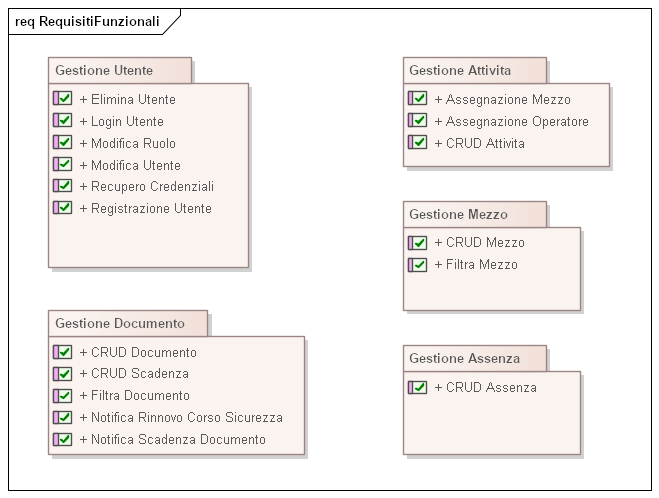
\includegraphics[width=1\textwidth]{immagini/RequisitiFunzionali.jpg}
\end{figure}
\begin{figure}[h!]
  \centering
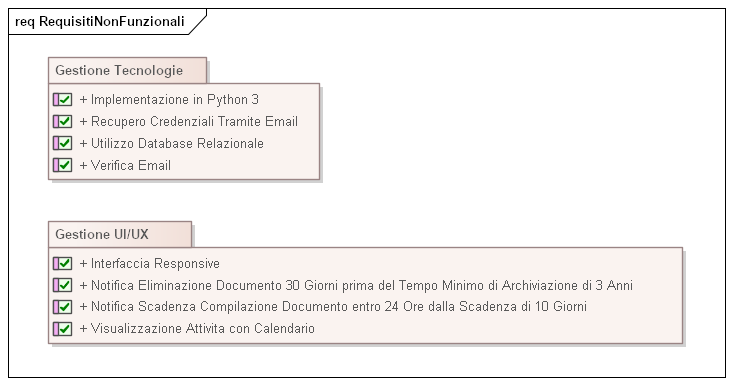
\includegraphics[width=0.7\textwidth]{immagini/RequisitiNonFunzionali.jpg}
\end{figure}
\newpage

\section{Tabella MoSCoW dei Requisiti}
\begin{table}[!ht]
\centering
\renewcommand\arraystretch{1.4}
\begin{tabular}{|p{3.5cm}|p{3.5cm}|p{3cm}|p{3cm}|}
\hline
\textbf{PRIORITÀ} & \textbf{ATTORE} & \textbf{AZIONE} & \textbf{TIPO} \\
\hline
\textbf{Must have} & Professore   & Prenotare aula                  & Funzionale \\ \cline{2-4}
                   & Professore   & Eliminare prenotazione          & Funzionale \\ \cline{2-4}
                   & Professore   & Gestire materiali/strumenti     & Funzionale \\ \cline{2-4}
                   & Ricercatore  & Prenotare aula                  & Funzionale \\ \cline{2-4}
                   & Ricercatore  & Eliminare prenotazione          & Funzionale \\ \cline{2-4}
                   & Tecnico      & Gestire inventario              & Funzionale \\ \cline{2-4}
                   & Studente     & Iscriversi ai corsi             & Funzionale \\ \cline{2-4}
                   & Studente     & Prenotare esperimenti           & Funzionale \\ \cline{2-4}
                   & Sistema      & Prenotazioni max 7gg prima      & Vincolo    \\ \cline{2-4}
                   & Sistema      & Disdette entro 2gg              & Vincolo    \\ 
\hline
\textbf{Should have} & Professore & Note personali                  & Funzionale \\ \cline{2-4}
                    & Professore & Gestione classi                 & Funzionale \\ \cline{2-4}
                    & Studente   & Disiscriversi dai corsi         & Funzionale \\ \cline{2-4}
                    & Sistema    & Log attività                    & Funzionale \\ \cline{2-4}
                    & Sistema    & Report danni strumenti          & Funzionale \\ 
\hline
\textbf{Could have} & Sistema    & Notifiche automatiche           & Funzionale \\ 
\hline
\textbf{Want to have} & Sistema  & App mobile                      & Funzionale     \\ 
\hline
\end{tabular}
\caption{Tabella dei requisiti secondo il metodo MoSCoW}
\end{table}
\newpage

\section{Diagrammi dei casi d'uso}
\subsubsection{Diagramma degli attori}
Il diagramma mette in evidenza gli attori che interagiscono con il sistema e le relazioni di eridarietà tra quest'ultimi.\\
\begin{figure}[h!]
  \centering
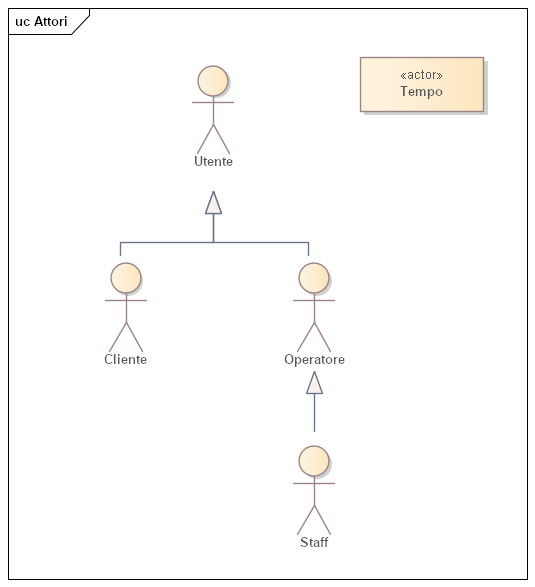
\includegraphics[width=1\textwidth]{immagini/Attori.jpg}
\end{figure}



\subsubsection{Gestione attività}
Il diagramma evidenzia le relazioni tra attori e casi d'uso per la gestione della tipologia di prenotazione: attività.\\
\begin{figure}[h!]
  \centering
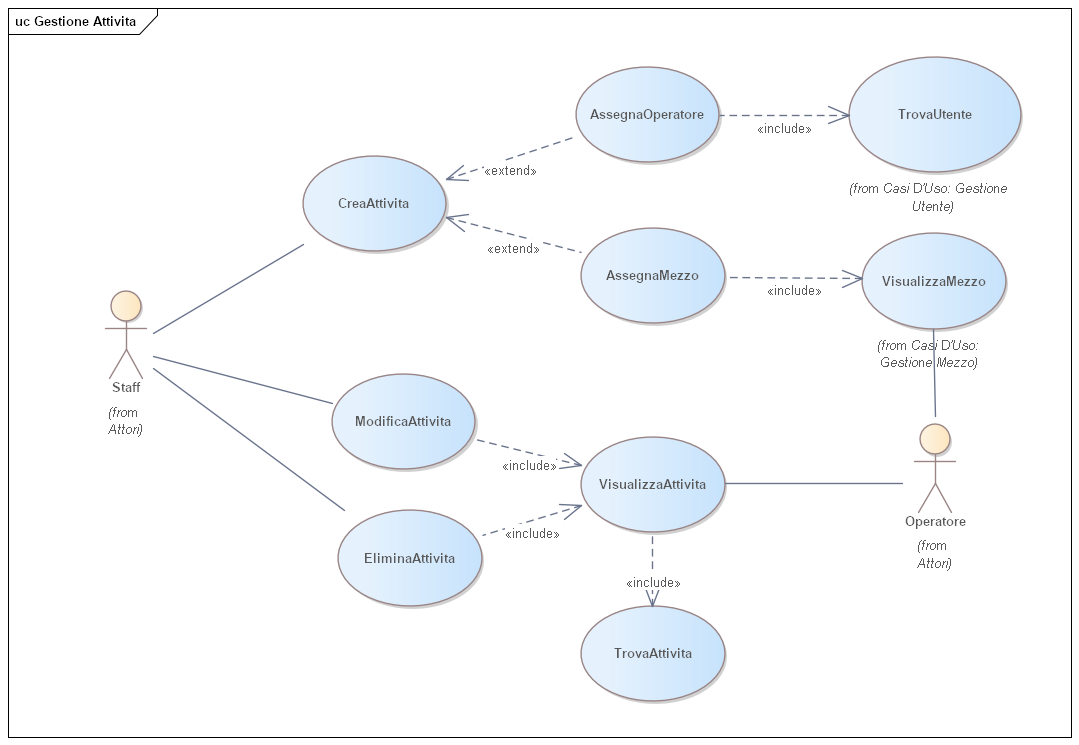
\includegraphics[width=1\textwidth]{immagini/GestioneAttivita.jpg}
\end{figure}
\newpage

%inserisciAttivita

\begin{table}[h!]
\centering
\renewcommand{\arraystretch}{1.3}
\begin{tabular}{|p{4.2cm}|p{10.2cm}|}
\hline
\multicolumn{2}{|c|}{\textbf{Caso d’uso: InserisciAttivita}} \\ \hline
\textbf{ID} & 1 \\ \hline
\textbf{Breve descrizione} & Il ricercatore inserisce una nuova attività \\ \hline
\textbf{Attori primari} & Ricercatore \\ \hline
\textbf{Attori secondari} & Nessuno \\ \hline
\textbf{Precondizioni} & Il ricercatore è stato autenticato dal sistema \\ \hline
\textbf{Sequenza degli eventi principale} &
1. Il caso d’uso inizia quando l'attore primario seleziona l’opzione “Inserisci nuova attività” \newline
2. L'attore primario aggiunge i dettagli: titolo, data, ora inizio, ora fine \newline
3. \texttt{If} la data odierna precede la data scelta di almeno 5 giorni \newline
\hspace*{1cm} 3.1 Il sistema controlla che per l’orario indicato non siano presenti altre prenotazioni \newline
\hspace*{1cm} 3.2 \texttt{If} sono presenti altre prenotazioni nello stesso intervallo \newline
\hspace*{1.5cm} 3.2.1 Il sistema mostra un messaggio di errore per indicare che la prenotazione non può essere effettuata \newline
\hspace*{1cm} 3.3 \texttt{Else} \newline
\hspace*{1cm} Punto di estensione: IndicaCapienzaMassima \newline
\hspace*{1.5cm} 3.3.1 Il sistema registra la prenotazione \newline
\hspace*{1.5cm} 3.3.2 Il sistema mostra un messaggio di conferma di avvenuta prenotazione \newline
4. \texttt{Else} \newline
\hspace*{0.5cm} 4.1 Il Sistema mostra un messaggio di errore che indica che la prenotazione non può essere effettuata (deve essere effettuata prima dei 5 giorni antecedenti alla data di prenotazione) \\ \hline
\textbf{Postcondizioni} & La lezione viene aggiunta al calendario \\ \hline
\textbf{Sequenza degli eventi alternativa} & Nessuno \\ \hline
\end{tabular}
\end{table}

\newpage


%modifica attività

\begin{table}[h!]
\centering
\renewcommand{\arraystretch}{1.3}
\begin{tabular}{|p{4.2cm}|p{10.2cm}|}
\hline
\multicolumn{2}{|c|}{\textbf{Caso d’uso:  ModificaAttivita}} \\ \hline
\textbf{ID} & 2 \\ \hline
\textbf{Breve descrizione} & Il ricercatore modifica un'attività \\ \hline
\textbf{Attori primari} & Ricercatore \\ \hline
\textbf{Attori secondari} & Nessuno \\ \hline
\textbf{Precondizioni} & 
1. Il ricercatore è stato autenticato dal sistema \newline
2. L'attività è stata inserita dal ricercatore \\ \hline
\textbf{Sequenza degli eventi principale} &
1. Il caso d’uso inizia quando il ricercatore seleziona l'attività che intende modificare \newline
2. \texttt{Include} (VisualizzaAttivita) \newline
3. Il ricercatore modifica i dati della l'attività \newline
4. \texttt{If} la nuova data è precedente alla vecchia data di almeno 3 giorni \newline
\hspace*{0.5cm} 4.1 Il sistema applica le modifiche apportate dal ricercatore \newline
5. \texttt{Else} \newline
\hspace*{0.5cm} 5.1 Il Sistema mostra un messaggio di errore che indica che non è più possibile apportare modifiche \\ \hline
\textbf{Postcondizioni} & L'attività viene aggiunta al calendario \\ \hline
\textbf{Sequenza degli eventi alternativa} & Nessuno \\ \hline
\end{tabular}
\end{table}
\newpage

%eliminaattività

\begin{table}[h!]
\centering
\renewcommand{\arraystretch}{1.3}
\begin{tabular}{|p{4.2cm}|p{10.2cm}|}
\hline
\multicolumn{2}{|c|}{\textbf{Caso d’uso: EliminaAttivita}} \\ \hline
\textbf{ID} & 3 \\ \hline
\textbf{Breve descrizione} & Il ricercatore elimina un'attività \\ \hline
\textbf{Attori primari} & Ricercatore \\ \hline
\textbf{Attori secondari} & Nessuno \\ \hline
\textbf{Precondizioni} &
1. Il ricercatore è stato autenticato dal sistema \newline
2. L'attivita è stata inserita dal ricercatore \\ \hline
\textbf{Sequenza degli eventi principale} &
1. Il caso d’uso inizia quando il ricercatore seleziona l'attività che intende eliminare \newline
2. \texttt{Include} (VisualizzaAttivita) \newline
3. Il ricercatore seleziona l’opzione “Elimina attività” \newline
4. \texttt{If} la data odierna è precedente a quella dell'attività di almeno 3 giorni \newline
\hspace*{0.5cm} 4.1 Il Sistema procede con la rimozione dell'attività \newline
\hspace*{0.5cm} 4.2 Il Sistema mostra un messaggio che indica che l'attività è stata eliminata \newline
5. \texttt{Else} \newline
\hspace*{0.5cm} 5.1 Il Sistema mostra un messaggio di errore che indica che non è possibile eliminare la prenotazione \\ \hline
\textbf{Postcondizioni} & L'attività viene rimossa dal calendario \\ \hline
\textbf{Sequenza degli eventi alternativa} & Nessuno \\ \hline
\end{tabular}
\end{table}

\space

%visualizzaattività

\begin{table}[h!]
\centering
\renewcommand{\arraystretch}{1.3}
\begin{tabular}{|p{4.2cm}|p{10.2cm}|}
\hline
\multicolumn{2}{|c|}{\textbf{Caso d’uso: VisualizzaAttivita}} \\ \hline
\textbf{ID} & 4 \\ \hline
\textbf{Breve descrizione} & Il sistema mostra i dettagli di un'attività \\ \hline
\textbf{Attori primari} & Studente, Ricercatore \\ \hline
\textbf{Attori secondari} & Nessuno \\ \hline
\textbf{Precondizioni} &
1. Lo Studente è stato autenticato dal sistema \newline
2. Il Ricercatore ha inserito l'attività \\ \hline
\textbf{Sequenza degli eventi principale} &
1. Il caso d’uso inizia quando l'attore principale seleziona l'attività che intende visualizzare \newline
2. Il Sistema mostra le informazioni relative all'attività \\ \hline
\textbf{Postcondizioni} & Nessuno \\ \hline
\textbf{Sequenza degli eventi alternativa} & Nessuno \\ \hline
\end{tabular}
\end{table}

\newpage

%iscrizioneattività

\begin{table}[h!]
\centering
\renewcommand{\arraystretch}{1.3}
\begin{tabular}{|p{4cm}|p{10cm}|}
\hline
\multicolumn{2}{|c|}{\textbf{Caso d’uso: IscrizioneAttivita}} \\ \hline
ID & 5 \\ \hline
Breve descrizione & Lo studente si iscrive ad un'attività \\ \hline
Attori primari & Studente \\ \hline
Attori secondari & Nessuno \\ \hline
Precondizioni &
1. Lo studente è stato autenticato dal sistema \newline
2. Il Ricercatore ha inserito l'attività \\ \hline
Sequenza degli eventi principale &
1. Il caso d’uso inizia quando lo Studente intende iscriversi ad un'attività \newline
2. \texttt{Include} (VisualizzaAttivita) \newline
3. Lo Studente seleziona l’opzione “Iscriviti” \newline
4. \texttt{If} Studente non è iscritto all'attività \newline
\hspace*{0.5cm} 4.1 \texttt{If} data odierna minore della data dell'attività di almeno 3 giorni \newline
\hspace*{1cm} 4.1.1 \texttt{If} il numero di persona non supera la capienza massima \newline
\hspace*{1.5cm} 4.1.1.1 Il Sistema inserisce lo Studente negli iscritti all'attività \newline
\hspace*{1.5cm} 4.1.1.2 Il Sistema mostra messaggio di conferma dell’iscrizione \newline
\hspace*{1cm} 4.1.2 \texttt{Else} \newline
\hspace*{1.5cm} 4.1.2.1 Il Sistema mostra un messaggio che segnala che la capienza è stata superata e non è possibile segnarsi \newline
\hspace*{0.5cm} 4.2 \texttt{Else} \newline
\hspace*{1cm} 4.2.1 Il Sistema segnala che non è più possibile iscriversi \newline
5. \texttt{Else} \newline
\hspace*{0.5cm} 5.1 Il Sistema mostra un messaggio di errore che indica che lo Studente è già segnato per la suddetta attività \\ \hline
Postcondizioni & Lo Studente è stato aggiunto agli iscritti dell'attività \\ \hline
Sequenza degli eventi alternativa & Nessuno \\ \hline
\end{tabular}
\end{table}
\newpage


%eliminaiscrizione attività

\begin{table}[h!]
\centering
\renewcommand{\arraystretch}{1.3}
\begin{tabular}{|p{4.2cm}|p{10.2cm}|}
\hline
\multicolumn{2}{|c|}{\textbf{Caso d’uso: EliminaIscrizioneAttivita}} \\ \hline
\textbf{ID} & 6 \\ \hline
\textbf{Breve descrizione} & Lo studente elimina una iscrizione ad un'attività \\ \hline
\textbf{Attori primari} & Studente \\ \hline
\textbf{Attori secondari} & Nessuno \\ \hline
\textbf{Precondizioni} &
1. Lo studente è stato autenticato dal sistema \newline
2. Lo Studente è iscritto all'attività \\ \hline
\textbf{Sequenza degli eventi principale} &
1. Il caso d’uso inizia quando lo Studente intende eliminare l'iscrizione ad un'attività \newline
2. \texttt{Include} (VisualizzaAttivita) \newline
3. Lo Studente seleziona l’opzione per disiscriversi dall'attività \newline
4. \texttt{If} Studente è iscritto \newline
\hspace*{0.5cm} 4.1 \texttt{If} data odierna è minore della data dell'attività di almeno un giorno \newline
\hspace*{1cm} 4.1.1 Il sistema rimuove lo Studente dagli iscritti dell'attività \newline
\hspace*{1cm} 4.1.2 Il Sistema mostra un messaggio che segnala l’eliminazione dell’iscrizione \newline
\hspace*{0.5cm} 4.2 \texttt{Else} \newline
\hspace*{1cm} 4.2.1 Il sistema segnala che la disdetta dell’iscrizione non può più essere effettuata \newline
5. \texttt{Else} \newline
\hspace*{0.5cm} 5.1 Il Sistema mostra un messaggio di errore \\ \hline
\textbf{Postcondizioni} & Lo Studente è stato rimosso dagli iscritti dell'attività \\ \hline
\textbf{Sequenza degli eventi alternativa} & Nessuno \\ \hline
\end{tabular}
\end{table}

\newpage




\subsubsection{Gestione lezione}
Il diagramma mette in evidenza le relazioni che intercorrono fra attori e casi d'uso al fine di realizzare le richieste legate alla tipologia 
di prenotazione: lezione. \\
\begin{figure}[h!]
  \centering
\includegraphics[width=1\textwidth]{immagini/Gestione Lezione.jpg}
\end{figure}

\newpage
% Caso d'uso: IscrizioneCorso
\begin{longtable}{|p{4cm}|p{10cm}|}
\hline
\multicolumn{2}{|c|}{\textbf{Caso d’uso: IscrizioneCorso}} \\
\hline
\textbf{ID:} & 7 \\
\hline
\textbf{Breve descrizione:} & Lo studente si iscrive ad un corso di un professore \\
\hline
\textbf{Attori primari:} & Studente \\
\hline
\textbf{Attori secondari:} & Professore \\
\hline
\textbf{Precondizioni:} & Lo studente è stato autenticato dal sistema \\
\hline
\textbf{Sequenza degli eventi principale:} &
\begin{itemize}[leftmargin=*, label={}]
  \item 1. Include (\textit{VisualizzaCorso})
  \item 2. Lo Studente seleziona “Iscriviti”
  \item 3. \texttt{If} Studente non è iscritto al corso:
  \begin{itemize}[leftmargin=1.5em, label={}]
    \item 3.1 Il Sistema aggiunge lo Studente agli iscritti del corso
    \item 3.2 \texttt{For} ogni lezione del corso
    \begin{itemize}[leftmargin=2em, label={}]
      \item 3.2.1 Include (\textit{IscrizioneLezione})
    \end{itemize}
  \end{itemize}
  \item 4. \texttt{Else}
  \begin{itemize}[leftmargin=1.5em, label={}]
    \item 4.1 Il Sistema mostra un messaggio di errore che segnala che lo Studente è già iscritto
  \end{itemize}
\end{itemize}
\\
\hline
\textbf{Postcondizioni:} & Lo Studente è stato aggiunto agli iscritti del corso \\
\hline
\textbf{Sequenza degli eventi alternativa:} & Nessuno \\
\hline
\end{longtable}


\newpage

% Caso d'uso: VisualizzaCorso
\begin{longtable}{|p{4cm}|p{10cm}|}
\hline
\multicolumn{2}{|c|}{\textbf{Caso d’uso: VisualizzaCorso}} \\
\hline
\textbf{ID} & 8 \\
\hline
\textbf{Breve descrizione} & Il Sistema mostra i dettagli di un corso \\
\hline
\textbf{Attori primari} & Studente, Professore \\
\hline
\textbf{Attori secondari} & Nessuno \\
\hline
\textbf{Precondizioni} & 
\begin{enumerate}[leftmargin=1em]
  \item Lo studente è stato autenticato dal sistema
  \item Il Professore è stato autenticato dal sistema
\end{enumerate} \\
\hline
\textbf{Sequenza degli eventi principale} & 
\begin{enumerate}[leftmargin=1em]
  \item Il caso d’uso inizia quando l’attore primario seleziona un corso
  \item Il Sistema mostra le seguenti informazioni: nome del corso, professore, descrizione
\end{enumerate}
Punto di estensione: \texttt{VisualizzaStudentiIscritti} \\
\hline
\textbf{Postcondizioni} & Nessuno \\
\hline
\textbf{Sequenza degli eventi alternativa} & Nessuno \\
\hline
\end{longtable}

%visualizzastudentiiscritti

\begin{table}[h!]
\centering
\renewcommand{\arraystretch}{1.3}
\begin{tabular}{|p{4.2cm}|p{10.2cm}|}
\hline
\multicolumn{2}{|c|}{\textbf{Caso d’uso di estensione: VisualizzaStudentiIscritti}} \\ \hline
\textbf{ID} & 9 \\ \hline
\textbf{Breve descrizione} & Segmento 1: Il Professore può visualizzare l’elenco degli studenti iscritti ad un suo corso \\ \hline
\textbf{Attori primari} & Professore \\ \hline
\textbf{Attori secondari} & Nessuno \\ \hline
\textbf{Precondizioni del segmento 1} &
1. Il Professore è stato autenticato dal sistema \newline
2. Il Professore ha selezionato un corso di cui visualizzare gli iscritti \\ \hline
\textbf{Sequenza degli eventi principale} &
1. Il caso d’uso inizia quando il professore seleziona l’opzione “Visualizza iscritti” \newline
2. Il sistema mostra l’elenco degli studenti iscritti al corso \\ \hline
\textbf{Postcondizioni} & Nessuno \\ \hline
\end{tabular}
\end{table}
\newpage

%eliminaiscrizionecorso

\begin{table}[h!]
\centering
\renewcommand{\arraystretch}{1.3}
\begin{tabular}{|p{4cm}|p{10cm}|}
\hline
\multicolumn{2}{|c|}{\textbf{Caso d’uso: EliminaIscrizioneCorso} }\\ \hline
\textbf{ID} & 10 \\ \hline
\textbf{Breve descrizione} & Lo studente si disiscrive da un determinato corso \\ \hline
\textbf{Attori primari} & Studente \\ \hline
\textbf{Attori secondari} & Nessuno \\ \hline
\textbf{Precondizioni} &
1. Lo studente è stato autenticato dal sistema \newline
2. Lo studente è iscritto al corso \\ \hline
\textbf{Sequenza degli eventi principale} &
1. Il caso d’uso inizia quando lo Studente intende eliminare l’iscrizione ad un corso \newline
2. \texttt{Include} (VisualizzaCorso) \newline
3. Lo Studente seleziona l’opzione per disiscriversi \newline
4. \texttt{If} Studente è iscritto al corso \newline
\hspace*{0.5cm} 4.1 Il Sistema mostra messaggio di conferma per disiscriversi \newline
\hspace*{0.5cm} 4.2 \texttt{If} il corso contiene lezioni \newline
\hspace*{1cm} 4.2.1 \texttt{For} ogni lezione del corso \newline
\hspace*{1.5cm} 4.2.1.1 \texttt{Include} (EliminaIscrizioneLezione) \newline
5. \texttt{Else} \newline
\hspace*{0.5cm} 4.1 Il Sistema mostra messaggio di errore che segnala che lo Studente non è iscritto \\ \hline
\textbf{Postcondizioni} & Lo Studente è rimosso dagli iscritti del corso \\ \hline
\textbf{Sequenza degli eventi alternativa} & Nessuno \\ \hline
\end{tabular}
\end{table}
\newpage

%iscrizionelezione

\begin{table}[h!]
\centering
\renewcommand{\arraystretch}{1.3}
\begin{tabular}{|p{4cm}|p{10cm}|}
\hline
\multicolumn{2}{|c|}{\textbf{Caso d’uso: IscrizioneLezione}} \\ \hline
ID & 11 \\ \hline
Breve descrizione & Lo studente si iscrive ad una lezione \\ \hline
Attori primari & Studente \\ \hline
Attori secondari & Nessuno \\ \hline
Precondizioni &
1. Lo studente è stato autenticato dal sistema \newline
2. Il Professore ha inserito la lezione \\ \hline
Sequenza degli eventi principale &
1. Il caso d’uso inizia quando lo Studente intende iscriversi alla lezione \newline
2. \texttt{Include} (VisualizzaLezione) \newline
3. Lo Studente seleziona l’opzione “Iscriviti” \newline
4. \texttt{If} Studente non è iscritto alla lezione \newline
\hspace*{0.5cm} 4.1 \texttt{If} data odierna minore della data della lezione di almeno 3 giorni \newline
\hspace*{1cm} 4.1.1 \texttt{If} il numero di persona non supera la capienza massima \newline
\hspace*{1.5cm} 4.1.1.1 Il Sistema inserisci lo Studente negli iscritti alla Lezione \newline
\hspace*{1.5cm} 4.1.1.2 Il Sistema mostra messaggio di conferma dell’iscrizione \newline
\hspace*{1cm} 4.1.2 \texttt{Else} \newline
\hspace*{1.5cm} 4.1.2.1 Il Sistema mostra un messaggio che segnala che la capienza è stata superata e non è possibile segnarsi \newline
\hspace*{0.5cm} 4.2 \texttt{Else} \newline
\hspace*{1cm} 4.2.1 Il Sistema segnala che non è più possibile iscriversi \newline
5. \texttt{Else} \newline
\hspace*{0.5cm} 5.1 Il Sistema mostra un messaggio di errore che indica che lo Studente è già segnato per la suddetta lezione \\ \hline
Postcondizioni & Lo Studente è stato aggiunto agli iscritti della lezione \\ \hline
Sequenza degli eventi alternativa & Nessuno \\ \hline
\end{tabular}
\end{table}
\newpage


%eliminaiscrizionelezione

\begin{table}[h!]
\centering
\renewcommand{\arraystretch}{1.3}
\begin{tabular}{|p{4.2cm}|p{10.2cm}|}
\hline
\multicolumn{2}{|c|}{\textbf{Caso d’uso: EliminaIscrizioneLezione}} \\ \hline
\textbf{ID} & 12 \\ \hline
\textbf{Breve descrizione} & Lo studente elimina un' iscrizione ad una lezione \\ \hline
\textbf{Attori primari} & Studente \\ \hline
\textbf{Attori secondari} & Nessuno \\ \hline
\textbf{Precondizioni} &
1. Lo studente è stato autenticato dal sistema \newline
2. Lo Studente è iscritto alla lezione \\ \hline
\textbf{Sequenza degli eventi principale} &
1. Il caso d’uso inizia quando lo Studente intende eliminare l'iscrizione ad una lezione \newline
2. \texttt{Include} (VisualizzaLezione) \newline
3. Lo Studente seleziona l’opzione per disiscriversi dalla lezione \newline
4. \texttt{If} Studente è iscritto \newline
\hspace*{0.5cm} 4.1 \texttt{If} data odierna è minore della data della lezione di almeno un giorno \newline
\hspace*{1cm} 4.1.1 Il sistema rimuove lo Studente dagli iscritti della lezione \newline
\hspace*{1cm} 4.1.2 Il Sistema mostra un messaggio che segnala l’eliminazione dell’iscrizione \newline
\hspace*{0.5cm} 4.2 \texttt{Else} \newline
\hspace*{1cm} 4.2.1 Il sistema segnala che la disdetta dell’iscrizione non può più essere effettuata \newline
5. \texttt{Else} \newline
\hspace*{0.5cm} 5.1 Il Sistema mostra un messaggio di errore \\ \hline
\textbf{Postcondizioni} & Lo Studente è stato rimosso dagli iscritti della lezione \\ \hline
\textbf{Sequenza degli eventi alternativa} & Nessuno \\ \hline
\end{tabular}
\end{table}

\space{}

%visualizzalezione

\begin{table}[h!]
\centering
\renewcommand{\arraystretch}{1.3}
\begin{tabular}{|p{4.2cm}|p{10.2cm}|}
\hline
\multicolumn{2}{|c|}{\textbf{Caso d’uso: VisualizzaLezione}} \\ \hline
\textbf{ID} & 13 \\ \hline
\textbf{Breve descrizione} & Il sistema mostra i dettagli di una lezione \\ \hline
\textbf{Attori primari} & Studente, Professore \\ \hline
\textbf{Attori secondari} & Nessuno \\ \hline
\textbf{Precondizioni} &
1. Lo studente è stato autenticato dal sistema \newline
2. Il Professore ha inserito la lezione \\ \hline
\textbf{Sequenza degli eventi principale} &
1. Il caso d’uso inizia quando l'attore principale seleziona la lezione che intende visualizzare \newline
2. Il Sistema mostra le informazioni relative alla leziona \\ \hline
\textbf{Postcondizioni} & Nessuno \\ \hline
\textbf{Sequenza degli eventi alternativa} & Nessuno \\ \hline
\end{tabular}
\end{table}

\newpage

%inseriscilezione

\begin{table}[h!]
\centering
\renewcommand{\arraystretch}{1.3}
\begin{tabular}{|p{4.2cm}|p{10.2cm}|}
\hline
\multicolumn{2}{|c|}{\textbf{Caso d’uso: InserisciLezione}} \\ \hline
\textbf{ID} & 14 \\ \hline
\textbf{Breve descrizione} & Il professore inserisce una nuova lezione \\ \hline
\textbf{Attori primari} & Professore \\ \hline
\textbf{Attori secondari} & Nessuno \\ \hline
\textbf{Precondizioni} & Il professore è stato autenticato dal sistema \\ \hline
\textbf{Sequenza degli eventi principale} &
1. Il caso d’uso inizia quando il professore vuole aggiungere una lezione \newline
2. Il professore seleziona l’opzione “Inserisci nuova lezione” \newline
3. Il professore aggiunge i dettagli: titolo, data, ora inizio, ora fine \newline
4. \texttt{If} la data odierna precede la data scelta di almeno 5 giorni \newline
\hspace*{0.5cm} 4.1 Il Sistema controlla che la lezione non abbia una durata superiore alle 2 ore \newline
\hspace*{0.5cm} 4.2 \texttt{If} durata della lezione minore delle 2 ore \newline
\hspace*{1cm} 4.2.1 Il sistema controlla che per l’orario indicato non siano presenti altre prenotazioni \newline
\hspace*{1cm} 4.2.2 \texttt{If} sono presenti altre prenotazioni nello stesso intervallo \newline
\hspace*{1.5cm} 4.2.2.1 Il sistema mostra un messaggio di errore per indicare che la prenotazione non può essere effettuata \newline
\hspace*{1cm} 4.2.3 \texttt{Else} \newline
\hspace*{1.5cm} 4.2.3.1 Il sistema registra la prenotazione \newline
\hspace*{1.5cm} 4.2.3.2 Il sistema mostra un messaggio di conferma di avvenuta prenotazione \newline
\hspace*{0.5cm} 4.3 \texttt{Else} \newline
\hspace*{1cm} 4.3.1 Il sistema mostra un messaggio di errore per indicare che la durata non può essere superiore alle due ore \newline
5. \texttt{Else} \newline
\hspace*{0.5cm} 5.1 Il Sistema mostra un messaggio di errore che indica che la prenotazione non può essere effettuata (deve essere effettuata prima dei 5 giorni antecedenti alla data di prenotazione) \\ \hline
\textbf{Postcondizioni} & La lezione viene aggiunta al calendario \\ \hline
\textbf{Sequenza degli eventi alternativa} & Nessuno \\ \hline
\end{tabular}
\end{table}

\newpage

%inseriscicorso

\begin{table}[h!]
\centering
\renewcommand{\arraystretch}{1.3}
\begin{tabular}{|p{4.2cm}|p{10.2cm}|}
\hline
\multicolumn{2}{|c|}{\textbf{Caso d’uso: InserisciCorso}} \\ \hline
\textbf{ID} & 15 \\ \hline
\textbf{Breve descrizione} & Il professore inserisce un nuovo corso \\ \hline
\textbf{Attori primari} & Professore \\ \hline
\textbf{Attori secondari} & Nessuno \\ \hline
\textbf{Precondizioni} &
1. Il professore è stato autenticato dal sistema \\ \hline
\textbf{Sequenza degli eventi principale} &
1. Il caso d’uso inizia quando il professore vuole aggiungere un corso \newline
2. Il professore seleziona l’opzione “Inserisci nuovo corso” \newline
3. Il professore aggiunge i dettagli: titolo, materia, professore, descrizione \newline
4. Il Sistema controlla che il corso non sia già presente nell’elenco dei corsi del professore \newline
5. \texttt{If} il corso è già presente \newline
\hspace*{0.5cm} 5.1 Il Sistema mostra un messaggio che indica che il corso è già presente \newline
6. \texttt{Else} \newline
\hspace*{0.5cm} 6.1 Il Sistema registra il nuovo corso e lo aggiunge all’elenco dei corsi del professore \newline
\hspace*{0.5cm} 6.2 Il Sistema mostra un messaggio che conferma l’inserimento del nuovo corso \\ \hline
\textbf{Postcondizioni} & Il corso viene aggiunto all’elenco dei corsi del professore \\ \hline
\textbf{Sequenza degli eventi alternativa} & Nessuno \\ \hline
\end{tabular}
\end{table}

%eliminacorso 

\begin{table}[h!]
\centering
\renewcommand{\arraystretch}{1.3}
\begin{tabular}{|p{4.2cm}|p{10.2cm}|}
\hline
\multicolumn{2}{|c|}{\textbf{Caso d’uso: EliminaCorso}} \\ \hline
\textbf{ID} & 16 \\ \hline
\textbf{Breve descrizione} & Il professore elimina un corso presente nel suo elenco dei corsi \\ \hline
\textbf{Attori primari} & Professore \\ \hline
\textbf{Attori secondari} & Nessuno \\ \hline
\textbf{Precondizioni} &
1. Il professore è stato autenticato dal sistema \newline
2. Il corso è presente all’interno dei corsi del professore \\ \hline
\textbf{Sequenza degli eventi principale} &
1. Il caso d’uso inizia quando il Professore seleziona il corso che intende eliminare \newline
2. \texttt{Include} (VisualizzaCorso) \newline
3. Il Professore seleziona l’opzione “Elimina corso” \newline
4. Il Sistema rimuove il corso dall’elenco dei corsi del professore \newline
5. Il Sistema mostra un messaggio di conferma di avvenuta rimozione del corso dall’elenco \\ \hline
\textbf{Postcondizioni} & Il corso viene rimosso dall’elenco dei corsi del professore \\ \hline
\textbf{Sequenza degli eventi alternativa} & Nessuno \\ \hline
\end{tabular}

\end{table}

\newpage

%modifica lezione

\begin{table}[h!]
\centering
\renewcommand{\arraystretch}{1.3}
\begin{tabular}{|p{4.2cm}|p{10.2cm}|}
\hline
\multicolumn{2}{|c|}{\textbf{Caso d’uso:  ModificaLezione}} \\ \hline
\textbf{ID} & 17 \\ \hline
\textbf{Breve descrizione} & Il professore modifica una lezione \\ \hline
\textbf{Attori primari} & Professore \\ \hline
\textbf{Attori secondari} & Nessuno \\ \hline
\textbf{Precondizioni} &
1. Il professore è stato autenticato dal sistema \newline
2. La lezione è stata inserita dal professore \\ \hline
\textbf{Sequenza degli eventi principale} &
1. Il caso d’uso inizia quando il professore seleziona la lezione che intende modificare \newline
2. \texttt{Include} (VisualizzaLezione) \newline
3. Il professore modifica i dati della lezione \newline
4. \texttt{If} la nuova data è precedente alla vecchia data di almeno 3 giorni \newline
\hspace*{0.5cm} 4.1 Il sistema applica le modifiche apportate dal professore \newline
5. \texttt{Else} \newline
\hspace*{0.5cm} 5.1 Il Sistema mostra un messaggio di errore che indica che non è più possibile apportare modifiche \\ \hline
\textbf{Postcondizioni} & La lezione viene aggiunta al calendario \\ \hline
\textbf{Sequenza degli eventi alternativa} & Nessuno \\ \hline
\end{tabular}
\end{table}

%eliminaprenotazionelezione

\begin{table}[h!]
\centering
\renewcommand{\arraystretch}{1.3}
\begin{tabular}{|p{4.2cm}|p{10.2cm}|}
\hline
\multicolumn{2}{|c|}{\textbf{Caso d’uso: EliminaPrenotazioneLezione}} \\ \hline
\textbf{ID} & 18 \\ \hline
\textbf{Breve descrizione} & Il professore elimina una lezione \\ \hline
\textbf{Attori primari} & Professore \\ \hline
\textbf{Attori secondari} & Nessuno \\ \hline
\textbf{Precondizioni} &
1. Il professore è stato autenticato dal sistema \newline
2. La lezione è stata inserita dal professore \\ \hline
\textbf{Sequenza degli eventi principale} &
1. Il caso d’uso inizia quando il professore seleziona la lezione che intende eliminare \newline
2. \texttt{Include} (VisualizzaLezione) \newline
3. Il professore seleziona l’opzione “Elimina lezione” \newline
4. \texttt{If} la data odierna è precedente a quella della lezione di almeno 3 giorni \newline
\hspace*{0.5cm} 4.1 Il Sistema procede con la rimozione della lezione \newline
\hspace*{0.5cm} 4.2 Il Sistema mostra un messaggio che indica che la lezione è stata eliminata \newline
5. \texttt{Else} \newline
\hspace*{0.5cm} 5.1 Il Sistema mostra un messaggio di errore che indica che non è possibile eliminare la prenotazione \\ \hline
\textbf{Postcondizioni} & La lezione viene rimossa dal calendario \\ \hline
\textbf{Sequenza degli eventi alternativa} & Nessuno \\ \hline
\end{tabular}
\end{table}

\newpage

\subsubsection{Gestione sistema}
Il diagramma mostra le relazioni fra attori e casi d'uso legate all'utente e alla gestione del back-up di sistema. \\
\begin{figure}[h!]
  \centering
\includegraphics[width=1\textwidth]{Gestione Sistema.jpg}
\end{figure}
\newpage

%backup
\begin{table}[htbp]
\centering
\begin{tabularx}{\textwidth}{|p{4cm}|X|}
\hline
\multicolumn{2}{|c|}{\textbf{Caso d'uso: Backup}}\\ \hline
\textbf{ID} & 19 \\ \hline
\textbf{Breve descrizione} & Il sistema esegue periodicamente il backup completo dei dati. \\ \hline
\textbf{Attori primari} & Tempo \\ \hline
\textbf{Attori secondari} & Sistema \\ \hline
\textbf{Precondizioni} & La pianificazione di backup è attiva e la finestra di manutenzione è disponibile. \\ \hline
\textbf{Sequenza degli eventi principale} &
\begin{minipage}[t]{\linewidth}
  \begin{enumerate}[label=\arabic*., leftmargin=*]
    \item Il caso d'uso inizia quando all’istante pianificato l’attore \emph{Tempo} innesca l’evento di backup.
    \item Il sistema crea un’istantanea del database e dei file critici.
    \item Il sistema copia l’istantanea su storage esterno.
    \item \textbf{If} (errore I/O o spazio insufficiente)
          \begin{enumerate}[label*=\arabic*., leftmargin=*]
            \item Il sistema registra l’errore.
          \end{enumerate}
    \item Il sistema registra nel log il completamento e marca l’ultimo backup come riuscito.
  \end{enumerate}
\end{minipage}\\ \hline
\textbf{Postcondizioni} & Snapshot di backup creato e registrato nel log. \\ \hline
\textbf{Sequenze degli eventi alternative} & Nessuno \\ \hline
\end{tabularx}
\end{table}

\newpage

%%%%%%%%%%%%%%%%%%%%%%%%%%%%%%%%%%%%%%%%%%%%%%%%%%%%%%%%%%%%%%%%%%%%%%%%%%%%%%
% UC-S2  Login
%%%%%%%%%%%%%%%%%%%%%%%%%%%%%%%%%%%%%%%%%%%%%%%%%%%%%%%%%%%%%%%%%%%%%%%%%%%%%%
\begin{table}[htbp]
\centering
\begin{tabularx}{\textwidth}{|p{4cm}|X|}
\hline
\multicolumn{2}{|c|}{\textbf{Caso d'uso: Login}}\\ \hline
\textbf{ID} & 20 \\ \hline
\textbf{Breve descrizione} & L’Utente si autentica per accedere alle funzionalità della piattaforma. \\ \hline
\textbf{Attori primari} & Utente \\ \hline
\textbf{Attori secondari} & Sistema \\ \hline
\textbf{Precondizioni} & 
\begin{minipage}[t]{\linewidth}
\begin{enumerate}[label=\arabic*., leftmargin=*]
  \item L’Utente è registrato
  \item La piattaforma non è in manutenzione.
\end{enumerate} 
\end{minipage}
\\ \hline
\textbf{Sequenza degli eventi principale} &
\begin{minipage}[t]{\linewidth}
  \begin{enumerate}[label=\arabic*., leftmargin=*]
    \item Il caso d'uso inizia quando l’Utente inserisce \emph{username} e \emph{password} e seleziona “Accedi”.
    \item Il sistema valida le credenziali.
    \item \textbf{If} (credenziali non valide)
          \begin{enumerate}[label*=\arabic*., leftmargin=*]
            \item Il sistema mostra “Login fallito” e registra il tentativo.
          \end{enumerate}
    \item Il sistema crea la sessione e reindirizza l’Utente alla home.
    \item Il sistema aggiorna il log di accesso.
  \end{enumerate}
\end{minipage}\\ \hline
\textbf{Postcondizioni} & Utente autenticato con sessione attiva. \\ \hline
\textbf{Sequenze degli eventi alternative} & Nessuno \\ \hline
\end{tabularx}
\end{table}

\newpage

%%%%%%%%%%%%%%%%%%%%%%%%%%%%%%%%%%%%%%%%%%%%%%%%%%%%%%%%%%%%%%%%%%%%%%%%%%%%%%
% UC-S3  InviaConferma
%%%%%%%%%%%%%%%%%%%%%%%%%%%%%%%%%%%%%%%%%%%%%%%%%%%%%%%%%%%%%%%%%%%%%%%%%%%%%%
\begin{table}[htbp]
\centering
\begin{tabularx}{\textwidth}{|p{4cm}|X|}
\hline
\multicolumn{2}{|c|}{\textbf{Caso d'uso: InviaConferma}}\\ \hline
\textbf{ID} & 21 \\ \hline
\textbf{Breve descrizione} & Il sistema invia e-mail o notifiche push di conferma e promemoria agli utenti. \\ \hline
\textbf{Attori primari} & Sistema \\ \hline
\textbf{Attori secondari} & Nessuno \\ \hline
\textbf{Precondizioni} & È avvenuto un evento che richiede una conferma (prenotazione, cancellazione, ecc.). \\ \hline
\textbf{Sequenza degli eventi principale} &
\begin{minipage}[t]{\linewidth}
  \begin{enumerate}[label=\arabic*., leftmargin=*]
    \item Il caso d'uso inizia quando il Sistema riceve l'iscrizione avvenuta ad un corso.
    \item Il Sistema compone il messaggio con i dati dell’evento.
    \item \textbf{If} (destinatario privo di indirizzo e-mail valido)
          \begin{enumerate}[label*=\arabic*., leftmargin=*]
            \item Il Sistema registra “Indirizzo mancante” e termina.
          \end{enumerate}
    \item Il Sistema invia il messaggio tramite e-mail o push.
    \item Il Sistema registra esito e timestamp nel log.
  \end{enumerate}
\end{minipage}\\ \hline
\textbf{Postcondizioni} & Conferma inviata oppure errore loggato e notificato. \\ \hline
\textbf{Sequenze degli eventi alternative} & Nessuno \\ \hline
\end{tabularx}
\end{table}

\newpage

\subsubsection{Gestione aula}
Il diagramma mette in evidenza le relazioni che interrono fra attori e casi d'uso per la gestione di materiali e strumenti del laboratorio. \\
\begin{figure}[h!]
  \centering
\includegraphics[width=1\textwidth]{Gestione Aula.jpg}
\end{figure}

\newpage
% UC-A1  InserisciMateriale
%=====================================================================
\begin{table}[htbp]
\centering
\begin{tabularx}{\textwidth}{|p{4cm}|X|}
\hline
\multicolumn{2}{|c|}{\textbf{Caso d'uso: InserisciMateriale}}\\ \hline
\textbf{ID} & 22 \\ \hline
\textbf{Breve descrizione} & Il Dipendente registra un nuovo materiale nel magazzino di laboratorio. \\ \hline
\textbf{Attori primari} & Dipendente (Professore, Ricercatore, Tecnico) \\ \hline
\textbf{Attori secondari} & Sistema \\ \hline
\textbf{Precondizioni} & Il Dipendente è autenticato e visualizza la pagina “Materiali”. \\ \hline
\textbf{Sequenza degli eventi principale} &
\begin{minipage}[t]{\linewidth}
  \begin{enumerate}[label=\arabic*., leftmargin=*]
    \item Il caso d'uso inizia quando il Dipendente seleziona \emph{Nuovo materiale}.
    \item Il sistema mostra il modulo di inserimento.
    \item Il Dipendente compila i campi obbligatori e conferma.
    \item \textbf{If} (codice materiale già presente)
          \begin{enumerate}[label*=\arabic*., leftmargin=*]
            \item Il sistema mostra un messaggio di errore che indica che la tipologia di materiale è già presente.
          \end{enumerate}
    \item Il sistema registra il materiale e ne visualizza il riepilogo.
  \end{enumerate}
\end{minipage}\\ \hline
\textbf{Postcondizioni} & Materiale inserito con stato “Disponibile”. \\ \hline
\textbf{Sequenze degli eventi alternative} & Nessuno \\ \hline
\end{tabularx}
\end{table}

\newpage

%=====================================================================
% UC-A2  ModificaMateriale
%=====================================================================
\begin{table}[htbp]
\centering
\begin{tabularx}{\textwidth}{|p{4cm}|X|}
\hline
\multicolumn{2}{|c|}{\textbf{Caso d'uso: ModificaMateriale}}\\ \hline
\textbf{ID} & 23 \\ \hline
\textbf{Breve descrizione} & Il Dipendente aggiorna descrizione o quantità di un materiale esistente. \\ \hline
\textbf{Attori primari} & Dipendente \\ \hline
\textbf{Attori secondari} & Sistema \\ \hline
\textbf{Precondizioni} & Il materiale è presente in inventario. \\ \hline
\textbf{Sequenza degli eventi principale} &
\begin{minipage}[t]{\linewidth}
  \begin{enumerate}[label=\arabic*., leftmargin=*]
    \item Il caso d'uso inizia quando il Dipendente seleziona \emph{Modifica} sul materiale.
    \item Il sistema mostra i campi editabili.
    \item Il Dipendente modifica i valori e conferma.
    \item \textbf{If} (quantità < 0)
          \begin{enumerate}[label*=\arabic*., leftmargin=*]
            \item Il sistema mostra un messaggio che inidica “Quantità non valida”.
          \end{enumerate}
    \item Il sistema salva le modifiche e aggiorna la scheda.
  \end{enumerate}
\end{minipage}\\ \hline
\textbf{Postcondizioni} & Scheda materiale aggiornata. \\ \hline
\textbf{Sequenze degli eventi alternative} & Nessuno \\ \hline
\end{tabularx}
\end{table}

\newpage

%=====================================================================
% UC-A3  EliminaMateriale
%=====================================================================
\begin{table}[htbp]
\centering
\begin{tabularx}{\textwidth}{|p{4cm}|X|}
\hline
\multicolumn{2}{|c|}{\textbf{Caso d'uso: EliminaMateriale}}\\ \hline
\textbf{ID} & 24 \\ \hline
\textbf{Breve descrizione} & Il Dipendente rimuove un materiale non più utilizzabile. \\ \hline
\textbf{Attori primari} & Dipendente \\ \hline
\textbf{Attori secondari} & Sistema \\ \hline
\textbf{Precondizioni} & Il materiale non è collegato a prenotazioni future. \\ \hline
\textbf{Sequenza degli eventi principale} &
\begin{minipage}[t]{\linewidth}
  \begin{enumerate}[label=\arabic*., leftmargin=*]
    \item Il caso d'uso inizia quando il Dipendente preme \emph{Elimina}.
    \item Il sistema chiede conferma.
    \item Il Dipendente conferma l’operazione.
    \item \textbf{If} (materiale prenotato in futuro)
          \begin{enumerate}[label*=\arabic*., leftmargin=*]
            \item Il sistema blocca l’operazione e mostra i riferimenti;
                  il caso d’uso termina.
          \end{enumerate}
    \item Il sistema sposta il materiale in stato “Rimosso” e aggiorna il log.
  \end{enumerate}
\end{minipage}\\ \hline
\textbf{Postcondizioni} & Materiale rimosso dal catalogo. \\ \hline
\textbf{Sequenze degli eventi alternative} & Nessuno \\ \hline
\end{tabularx}
\end{table}

\newpage

%=====================================================================
% UC-A4  InserisciStrumento
%=====================================================================
\begin{table}[htbp]
\centering
\begin{tabularx}{\textwidth}{|p{4cm}|X|}
\hline
\multicolumn{2}{|c|}{\textbf{Caso d'uso: InserisciStrumento}}\\ \hline
\textbf{ID} & 25 \\ \hline
\textbf{Breve descrizione} & Il Tecnico registra un nuovo strumento in laboratorio. \\ \hline
\textbf{Attori primari} & Tecnico \\ \hline
\textbf{Attori secondari} & Sistema \\ \hline
\textbf{Precondizioni} & Tecnico autenticato; pagina “Strumenti” aperta. \\ \hline
\textbf{Sequenza degli eventi principale} &
\begin{minipage}[t]{\linewidth}
  \begin{enumerate}[label=\arabic*., leftmargin=*]
    \item Il caso d'uso d'uso inizia quando il Tecnico seleziona \emph{Nuovo strumento}.
    \item Compila i dati obbligatori (codice, descrizione, quantità).
    \item \textbf{If} (codice duplicato)
          \begin{enumerate}[label*=\arabic*., leftmargin=*]
            \item Il sistema mostra un messagio di errore che indica “Codice già in uso”.
          \end{enumerate}
    \item Il sistema salva lo strumento e visualizza la scheda dettagliata.
  \end{enumerate}
\end{minipage}\\ \hline
\textbf{Postcondizioni} & Strumento aggiunto in inventario. \\ \hline
\textbf{Sequenze degli eventi alternative} & Nessuno\\ \hline
\end{tabularx}
\end{table}

\newpage

%=====================================================================
% UC-A5  ModificaStrumento
%=====================================================================
\begin{table}[htbp]
\centering
\begin{tabularx}{\textwidth}{|p{4cm}|X|}
\hline
\multicolumn{2}{|c|}{\textbf{Caso d'uso: ModificaStrumento}}\\ \hline
\textbf{ID} & 26 \\ \hline
\textbf{Breve descrizione} & Il Tecnico aggiorna informazioni o stato di uno strumento. \\ \hline
\textbf{Attori primari} & Tecnico \\ \hline
\textbf{Attori secondari} & Sistema \\ \hline
\textbf{Precondizioni} & Strumento esistente in inventario. \\ \hline
\textbf{Sequenza degli eventi principale} &
\begin{minipage}[t]{\linewidth}
  \begin{enumerate}[label=\arabic*., leftmargin=*]
    \item Il caso d'uso inizia quando il Tecnico seleziona \emph{Modifica}.
    \item Il sistema mostra i campi editabili.
    \item Il Tecnico modifica i valori e conferma.
    \item \textbf{If} (valori fuori range)
          \begin{enumerate}[label*=\arabic*., leftmargin=*]
            \item Il sistema mostra un messaggio di errore.
          \end{enumerate}
    \item Il sistema salva e visualizza la scheda aggiornata.
  \end{enumerate}
\end{minipage}\\ \hline
\textbf{Postcondizioni} & Scheda strumento aggiornata. \\ \hline
\textbf{Sequenze degli eventi alternative} & Nessuno \\ \hline
\end{tabularx}
\end{table}

\newpage

%=====================================================================
% UC-A6  EliminaStrumento
%=====================================================================
\begin{table}[htbp]
\centering
\begin{tabularx}{\textwidth}{|p{4cm}|X|}
\hline
\multicolumn{2}{|c|}{\textbf{Caso d'uso: EliminaStrumento}}\\ \hline
\textbf{ID} & 27 \\ \hline
\textbf{Breve descrizione} & Il Tecnico rimuove uno strumento danneggiato. \\ \hline
\textbf{Attori primari} & Tecnico \\ \hline
\textbf{Attori secondari} & Sistema \\ \hline
\textbf{Precondizioni} & Lo strumento è marcato “Non funzionante”. \\ \hline
\textbf{Sequenza degli eventi principale} &
\begin{minipage}[t]{\linewidth}
  \begin{enumerate}[label=\arabic*., leftmargin=*]
    \item Il caso d'uso inizia quando il Tecnico seleziona \emph{Elimina strumento}.
    \item \textbf{If} (strumento prenotato in futuro)
          \begin{enumerate}[label*=\arabic*., leftmargin=*]
            \item Il sistema blocca l’operazione, mostra le prenotazioni e termina.
          \end{enumerate}
    \item Il sistema rimuove lo strumento e aggiorna il log.
  \end{enumerate}
\end{minipage}\\ \hline
\textbf{Postcondizioni} & Inventario privo dello strumento eliminato. \\ \hline
\textbf{Sequenze degli eventi alternative} & Nessuno \\ \hline
\end{tabularx}
\end{table}

\newpage
%=====================================================================
% UC-A7  VisualizzaMateriale
%=====================================================================
\begin{table}[htbp]
\centering
\begin{tabularx}{\textwidth}{|p{4cm}|X|}
\hline
\multicolumn{2}{|c|}{\textbf{Caso d'uso: VisualizzaMateriale}}\\ \hline
\textbf{ID} & 28 \\ \hline
\textbf{Breve descrizione} & Il Dipendente consulta l’elenco dei materiali con filtri e stato. \\ \hline
\textbf{Attori primari} & Dipendente \\ \hline
\textbf{Attori secondari} & Sistema \\ \hline
\textbf{Precondizioni} & Dipendente autenticato. \\ \hline
\textbf{Sequenza degli eventi principale} &
\begin{minipage}[t]{\linewidth}
  \begin{enumerate}[label=\arabic*., leftmargin=*]
    \item Il Dipendente apre \emph{Visualizza materiali}.
    \item Il sistema mostra la tabella con filtri per nome, categoria, disponibilità.
  \end{enumerate}
\end{minipage}\\ \hline
\textbf{Postcondizioni} & Lista materiali visualizzata. \\ \hline
\textbf{Sequenze degli eventi alternative} & Nessuno \\ \hline
\end{tabularx}
\end{table}

\newpage

%=====================================================================
% UC-A8  VisualizzaStrumento
%=====================================================================
\begin{table}[htbp]
\centering
\begin{tabularx}{\textwidth}{|p{4cm}|X|}
\hline
\multicolumn{2}{|c|}{\textbf{Caso d'uso: VisualizzaStrumento}}\\ \hline
\textbf{ID} & 29 \\ \hline
\textbf{Breve descrizione} & Il Dipendente consulta l’elenco degli strumenti con dettaglio stato. \\ \hline
\textbf{Attori primari} & Dipendente \\ \hline
\textbf{Attori secondari} & Sistema \\ \hline
\textbf{Precondizioni} & Dipendente autenticato. \\ \hline
\textbf{Sequenza degli eventi principale} &
\begin{minipage}[t]{\linewidth}
  \begin{enumerate}[label=\arabic*., leftmargin=*]
    \item Il Dipendente apre \emph{Visualizza strumenti}.
    \item Il sistema mostra elenco strumenti con filtri e disponibilità in tempo reale.
  \end{enumerate}
\end{minipage}\\ \hline
\textbf{Postcondizioni} & Lista strumenti visualizzata. \\ \hline
\textbf{Sequenze degli eventi alternative} & Nessuno \\ \hline
\end{tabularx}
\end{table}
\newpage

\section{Matrice di Mapping}
\includegraphics[width=1\textwidth]{MappadeiRequisiti.png}\newpage
\chapter{Analisi}
La sequente sezione è dedicata al flusso di lavoro dell'analisi. In quest'ultima sono stati inseriti:
\begin{itemize}
  \item il diagramma dei package di analisi 
  \item i diagrammmi delle classi di analisi
  \item i diagrammi di sequenza, come parte della realizzazione dei casi d'uso, con lo scopo di mettere in evidenza le relazioni che intercorrono tra oggetti che realizzano il caso d'uso
  \item i diagrammi di attività, con l'intento di evidenziare il processo dei casi d'uso
\end{itemize}

\section{Diagrammi delle classi di analisi}
\subsection{Package di analisi}

\begin{figure}[htbp]
    \centering
    \includegraphics[width=0.8\textwidth]{packageAnalisi.jpg} % o .png, .jpeg, .pdf
    \caption{Diagramma dei package di analisi}
    \label{fig:etichetta}
\end{figure}
\newpage

\subsection{Package di Analisi: Utente}
Il diagramma ha lo scopo di evidenziare la relazione di ereditarietà fra l'utente e le varie tipologie di ruoli che posso eseguire all'accesso al sistema. 
\begin{figure}[htbp]
    \centering
    \includegraphics[width=0.9\textwidth]{UtenteAnalisi.jpg} % o .png, .jpeg, .pdf
\end{figure}
\newpage

\subsection{Package di Analisi: Aula}
Il diagramma mette in evidenza la struttura statica, in particolare le relazioni presenti fra le varie tipologie di utente e gli elementi che possono gestire all'interno del sistema. 
\begin{figure}[htbp]
    \centering
    \includegraphics[width=1.1\textwidth]{AulaAnalisi.jpg} % o .png, .jpeg, .pdf
\end{figure}
\newpage

\section{Diagrammi di sequenza}
\subsection{Corso CD}
Il diagramma mostra il flusso di iterazione fra i vari elementi di modellazione per la creazione e rimozione di un corso effettuato dal professore. 
\begin{figure}[htbp]
    \centering
    \includegraphics[width=0.7\textwidth]{CorsoCD.jpg} % o .png, .jpeg, .pdf
\end{figure}
\newpage

\subsection{Iscrizione Corso CD}
Il diagramma mostra il flusso di interazioni tra uno studente e i componenti del sistema coinvolti nel processo di iscrizione e disiscrizione da un corso, con eventuali iscrizioni e disiscrizioni automatiche alle lezioni correlate.
\begin{figure}[h!]
  \centering
\includegraphics[width=0.8\textwidth]{IscrizioneCorsoCD.jpg}
\end{figure}
\newpage

\subsection{Iscrizione Lezione}
Il diagramma mostra il flusso di interazione tra lo studenti e i componenti del sistema coinvolti nel processo di iscrizione e disiscrizione da una prenotazione, di entrambe le tipologie: Attività e Lezione. 
\begin{figure}[h!]
  \centering
\includegraphics[width=0.6\textwidth]{Iscrizione.jpg}
\end{figure}

\newpage

\subsection{Strumento CUD}
Il diagramma mostra il flusso di interazione del tecnico e i componenti del sistema nel processo di aggiunta, modifica o rimozione di uno strumento (in maniera analoga può essere gestiro il flusso di creazione, modifica e rimozione di Materiale).
\begin{figure}[h!]
  \centering
\includegraphics[width=0.7\textwidth]{StrumentoCUD.jpg}
\end{figure}
\newpage

\subsection{Prenotazione CUD}
Il diagramma mostra il flusso di interazione fra il ricercatore o professore e vari componenti del sistema nel processo per aggiungere, modificare e rimuoreve un attività (il processo per aggiungere, modificare e rimuovere una prenotazione del tipo lezione da parte del professore può eddere modellato in maniera analoga).
\begin{figure}[h!]
  \centering
\includegraphics[width=0.6\textwidth]{PrenotazioneCUD.jpg}
\end{figure}
\newpage

\subsection{Utente Login}
Il diagramma mette in evidenza il processo di accesso dell'utente al sistema. In particolare mostra la validazione delle credenziali da parte di un sistema esterno e il reindirizzamento in base alla tipologia di utente. 
\begin{figure}[h!]
  \centering
\includegraphics[width=1\textwidth]{UtenteLogin.jpg}
\end{figure}
\newpage


\section{Diagrammi di attività}
\subsection{Corso CD}
Il seguente diagramma di attività gestisce il processo di creazione e rimozione di un corso tramite flusso di azioni.In particolare un nodo azione (il nodo azione di chiamata) può attivare: un attività, un comportamento, un'operazione. In questo caso Ricerca Corso richiama un'altra attività (si utilizza il simbolo del rastrello). Inoltre è stato utilizzato un nodo oggetto per indicare la crezione di un nuovo Corso. 

\begin{figure}[h!]
  \centering
  \includegraphics[width=1\textwidth]{CorsoCDAttivita.jpg}
\end{figure}
\newpage
\subsection{Iscrizione Corso CD}
Il diagramma mostra l'iscrizione e la disiscrizione di uno studente da un corso modellando l'attività tramite un flusso di azioni. 

\begin{figure}[h!]
  \centering
  \includegraphics[width=1\textwidth]{IscrizioneCorsoCDAttivita.jpg}
\end{figure}
\newpage

\subsection{Iscrizione Lezione}
Il diagramma modella il caso d'uso IscrizioneLezione fornendo una forma più compatta come serie di azioni. 

\begin{figure}[h!]
  \centering
  \includegraphics[width=1\textwidth]{IscrizioneLezioneAttivita.jpg}
\end{figure}
\newpage

\subsection{Strumento CUD}
Il diagramma mostra la creazione, modifica e rimozione di uno Strumento. La creazione, modifica e rimozione di Materiale può essere trattata in maniera analoga.

\begin{figure}[h!]
  \centering
  \includegraphics[width=1\textwidth]{StrumentoCUDAttivita.jpg}
\end{figure}
\newpage

\subsection{Prenotazione CUD}
Il diagramma mostra il processo di creazione, modifica e rimozione di una prenotazione tramite un flusso di azioni. 

\begin{figure}[h!]
  \centering
  \includegraphics[width=1\textwidth]{PrenotazioneCUDAttivita.jpg}
\end{figure}
\newpage


\chapter{Progettazione}
La seguente sezioni è dedicata al flusso di lavoro della Progettazione. Infatti sono stati inseriti:
\begin{itemize}
  \item il diagramma dei package
  \item i diagrammi delle classi di progettazione
  \item il diagramma dei componenti
  \item i diagrammi delle macchine a stati
\end{itemize}
Il diagramma dei package è stato ripreso dal diagramma dei package di analisi, nella fase di progettazione un unico package può essere convertito in diversi sottosistemi di progettazione.\\
I diagrammi delle classi di analisi sono stati ripresi e ampliati allo scopo di essere classi complete utili come base per l'implementazione. Al fine di assolvere alle loro responsabilità: è stato completato l'insieme degli attributi, includendo tutte le specifiche; 
è stato completato l'insieme delle operazioni, convertendo una singola operazione dell'analisi in uno o più metodi. 
Una classe di analisi può essere convertita in una o più classi di progettazione o interfacce. A tal scopo è stato aggiunto un ulteriore diagramma per le classi.\\
Per descrivere le relazioni fra i vari componenti è stato utilizzato un diagramma dei componenti.\\
All'interno della progettazione è possibile ampliare i diagrammi di sequenza. Sono stati aggiunti nella sezione progettazione i diagrammi delle macchine a state, con scopo e semantica differrenti modellano anch'esse come i diagrammi dell'analisi il comportamento dinamico del sistema. 
Le macchine a stati sono utili per modellare il ciclo di vita dell'oggetto. 


\section{Diagrammi delle classi di progettazione}
\section{Diagrammi delle macchine a stati}
\section{Diagrammi dei componenti}




\chapter{Implementazione}
La seguente sezione è dedicata al flusso di lavoro dell'implementazione, nella quale sono stati inseriti: il diagramma di deployment, una descrizione delle tecnologie utilizzate, 
il mockup ed infine la descrizione unit test. 
\section{Diagrammi di deployment}
\begin{figure}[h!]
  \centering
  \includegraphics[width=0.7\textwidth]{Implementazione.jpg}
\end{figure}
\newpage

\section{Tecnologie utilizzate}
\subsection{Tecnologie Front-End}
\subsubsection{Flask Template}
Flask è un web framework open source scritto con Python caratterizzato da flessibilità, leggerezza e semplicità d'uso.\\
\subsubsection{CSS, Javascript e HTML}
Queste Tecnologie vengono utilizzate per la parte visuale e per rendere il sito più dinamico. CSS è un linguaggio utilizzato per descrivere
l'aspetto e la formattazione di una pagina web realizzata tramite HTML.\\
Il linguaggio HTML è usato per definire la struttura della pagina (testi, titoli, immagini ecc...).\\
Infine Javascript, un linguaggio lato client usato per rendere le pagine web interattive; permette al sito di rispondere alle azioni dell'utente (ad esempio: click, digitazione, scroll...). 
\subsection{Tecnologie Back-End}
\subsubsection{SQLite}
SQLite
è una libreria software scritta in linguaggio C che implementa il DBMS (DataBase Management System), dove abbiamo salvato diversi dati tra cui gli utenti:\newline
"S1119045","Ronchini Davide","pwd","professore",\newline
 "S1119245","Rossi Mario","pwd","studente",\newline
 "S1119345","Verdi Giuseppe","pwd","tecnico",\newline
 "S1119545","Bianchi Luigi","pwd","ricercatore"\newline
Si tratta di un database relazionale leggero contenuto in un unico file di tipo .db, che non necessita di un server esterno. 
Si adatta perfettamente ad app web realizzate con Flask e ai moderni linguaggi di programmazione, incluso Python.
\subsubsection{Flask}
Flask è utilizzato per realizzare applicazioni web in Python. Non sono necessarie particolari librerie per poterlo utilizzare.
\subsection{Tecnologie Versione Control System}
\subsubsection{GitHub}
GitHub è una piattaforma online per il versionamento del codice sorgente e la collaborazione tra sviluppatori, basata su Git, un sistema di controllo di versione distribuito.
La repository Git permette di gestire progetti con il loro storico delle modifiche. 
Quindi ci ha consetito di sviluppare le funzionalità del progetto in parallelo, garantendo la sincronizzazione
continua del codice, oltre che fornire un backup sicuro e centralizzato.
\subsection{Altre tecnologie utilizzate}
\subsubsection{Enterprise Architect}
Enterprise Architect (EA) è uno strumento utilizzato per la modellazione, progettazione, documentazione e gestione di sistemi software, architetture aziendali e processi complessi.
All'interno del progetto è stato usato per generare i diagrammi in UML che costituiscono la base dell'intera archittetura della piattaforma web, supportando 
tutto il ciclo di vita di realizzazione a partire dai requisiti sino all'implementazione. 

\section{Mockup}
\subsection{Pagina principale}
\begin{figure}[h!]
  \centering
\includegraphics[width=1\textwidth]{Home Page1.png}
\end{figure}
\newpage

\subsection{Pagina vista sul calendario delle prenotazioni}
\begin{figure}[h!]
  \centering
\includegraphics[width=1\textwidth]{Home Page2.png}
\end{figure}

\newpage

\subsection{Pagina per inserimento prenotazione}
\begin{figure}[h!]
  \centering
\includegraphics[width=1\textwidth]{Home Page3.png}
\end{figure}
\newpage

\subsection{Pagina vista del tecnico}
\begin{figure}[h!]
  \centering
\includegraphics[width=0.9\textwidth]{Home Page4.png}
\end{figure}
\newpage

\subsection{Pagina vista sui corsi}
\begin{figure}[h!]
  \centering
\includegraphics[width=1\textwidth]{Home Page6.png}
\end{figure}
\newpage

\section{Prerequisiti}
Per poter eseguire correttamente il progetto o l'applicazione, è necessario che sul tuo computer siano presenti i seguenti strumenti 
e componenti software:
\paragraph{Python 3 (o versione successiva)}
È necessario avere installata una versione di Python pari o superiore alla 3.
Per verificare se Python è installato e controllarne la versione, apri il terminale (o prompt dei comandi) e digita:\\
\texttt{python --version}\\
Se il comando restituisce una versione (es. Python 3.11.5), allora Python è correttamente installato. In caso contrario, 
dovrai scaricarlo dal sito ufficiale: https://www.python.org/downloads/.\\
\paragraph{Pip – il gestore di pacchetti di Python}
Pip è lo strumento che consente di installare e gestire le librerie Python.
È normalmente incluso nelle versioni recenti di Python, ma puoi verificarne la presenza digitando nel terminale:\\
\texttt{pip --version}\\
Se pip non è installato, puoi seguire le istruzioni ufficiali su: https://pip.pypa.io/en/stable/installation/.\\
\paragraph{Virtualenv – per creare ambienti virtuali Python isolati}
Virtualenv è un modulo Python che consente di creare ambienti virtuali indipendenti, utili per gestire le dipendenze di un progetto 
senza interferenze con altri progetti o con l'ambiente Python globale.
Per verificare se è installato, puoi provare il comando:\\
\texttt{virtualenv --version}\\
Se non è installato, puoi aggiungerlo al tuo sistema tramite pip con il comando:\\
\texttt{pip install virtualenv}
\newpage
\section{Descrizione unit test}

\cleardoublepage
\addcontentsline{toc}{chapter}{Bibliografia}
\bibliographystyle{plain}
\bibliography{bibliografia}









\end{document}